\section{Problem}

Centralized systems as the name suggests are systems where one primary system manages all computing resources. In spite of the benefits of centralized systems such as small capital and operational cost (minimum hardware) they are often faced with problems such as single point failure, limited scalability, computational bottleneck, fault tolerance and so on. Thus centralized systems are unsuitable for many large real world applications.

In the Simple Shared Dictionary Compression for Publisher-Subscriber (SSPS) model, the entity called Sampling Broker(SB) is responsible for sampling notifications to create dictionaries, maintaining the dictionary and spreading the dictionary to the publishers and subscribers. To the best of our knowledge currently the only implementation of SSPS exists on one centralized broker called Moquette \parencite{moquette}. However, one of the major drawbacks is that this sampling broker is a centralized entity and hence it is prone to all the disadvantages of a centralized system.

\makeatletter
\setlength{\@fptop}{0pt}
\makeatother

\begin{figure}[t!]
\centering
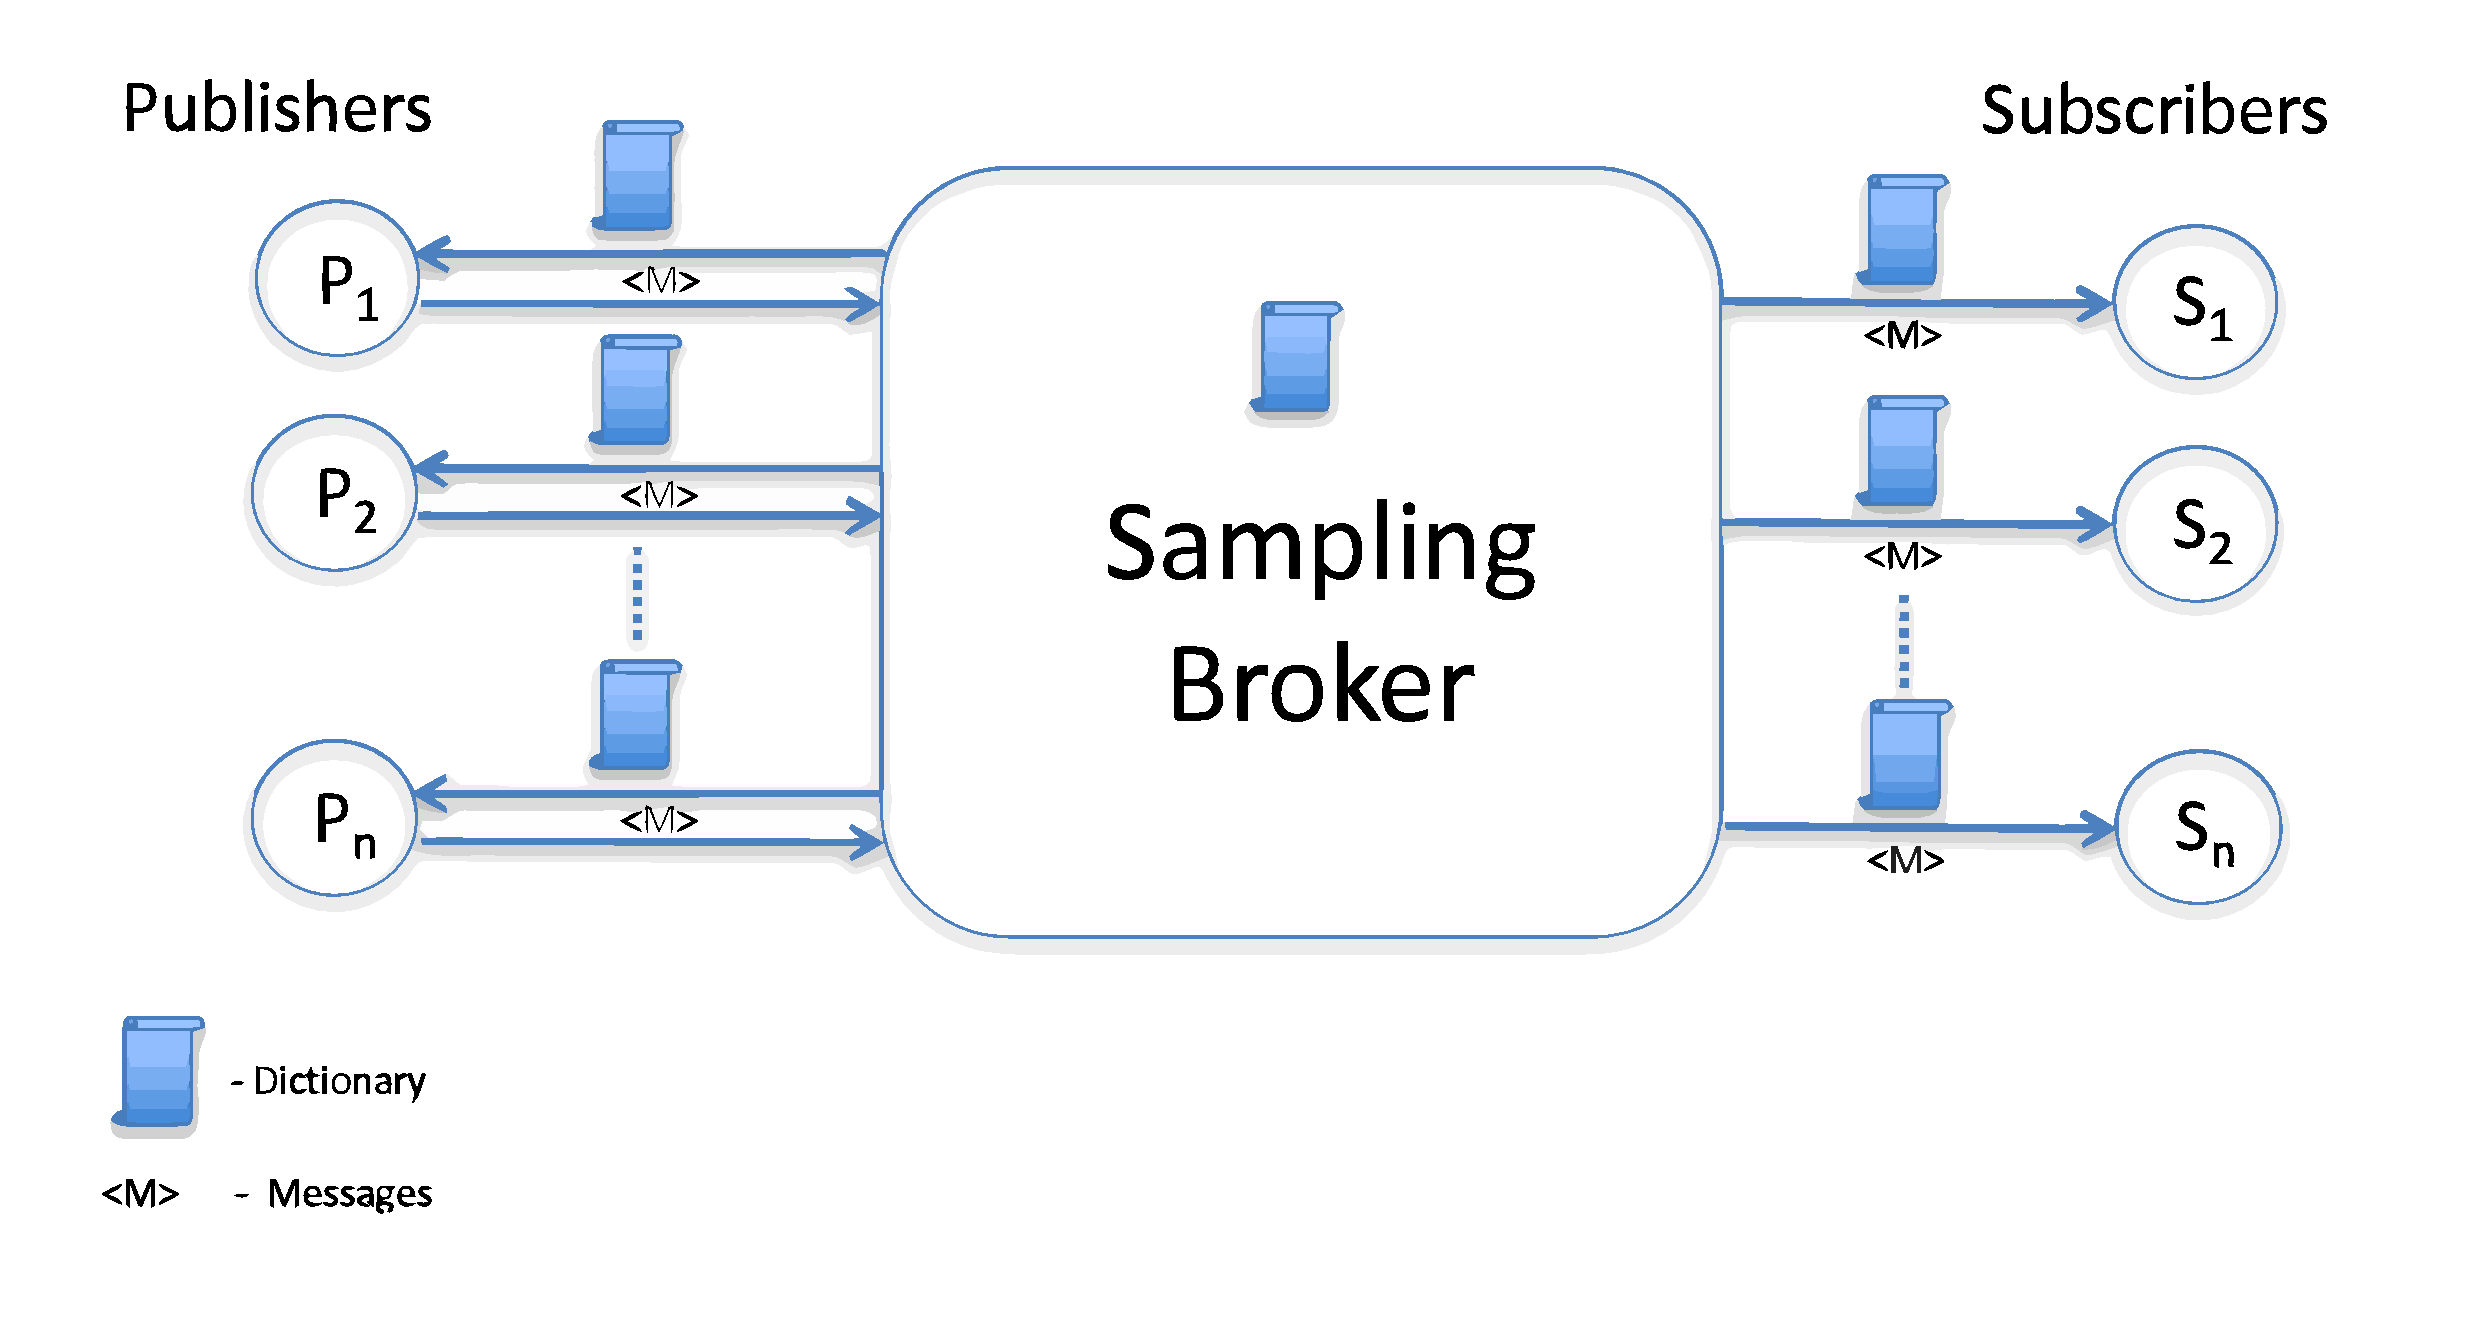
\includegraphics[keepaspectratio, width=.9\textwidth, trim={0 12cm 0 9cm},clip]{ssps.pdf}
\caption{Sampling Broker in SSPS model}\label{figures:ssps}
\end{figure}

Figure \ref{figures:ssps} depicts the current state of the art implementation of the Sampling Broker of the SSPS model. As the number of publishers and subscribers increase, there would be a computational bottleneck. Also in the case of failure, the entire SSPS model would collapse, which is not desirable in the real world. Thus, there is a need to overcome the problem of this centralized entity. 
